\documentclass[a4paper,10pt,onecolumn,preprint,3p]{elsarticle}

\usepackage{graphics,subfigure}
\usepackage{amssymb}
\usepackage{amsmath}
\usepackage[dvips]{epsfig}
\usepackage[latin1]{inputenc}
\usepackage{url}

\def\CC{{C\hspace{-.05em}\raisebox{.4ex}{\tiny\bf ++}}~}
\addtolength{\textfloatsep}{-0.5cm}
\addtolength{\intextsep}{-0.5cm}

\journal{Journal of XXX}

\begin{document}

%\begin{frontmatter}

%%%%%%%%%%%%%%%% Title %%%%%%%%%%%%%%%
\title{Predicting Levels of Sales for Newly Published Books \\
using Cost-Sensitive Ensemble Methods}


%%%%%%%%%%%%%%%% Authors %%%%%%%%%%%%%%
\author[abd]{Hossam Faris}
\ead{hossam.faris@ju.edu.jo}
\author[ugrtstc]{Antonio M. Mora}
\ead{amorag@geneura.ugr.es}
\author[ugratc]{Pedro A. Castillo}
\ead{pacv@ugr.es}
\author[ugratc]{J.J. Merelo}
\ead{jmerelo@geneura.ugr.es}
%\author[ugratc]{Pablo Garc\'{\i}a-S\'anchez}
%\ead{pablogarcia@ugr.es}


\address[abd]{Business Information Technology Department, King Abdullah II School for Information Technology \\
The University of Jordan, Amman, Jordan}
\address[ugrtstc]{Department of Signal Theory, Telematics and Communications, ETSIIT and CITIC \\
University of Granada, Granada, Spain}
\address[ugratc]{Department of Computer Architecture and Computer Technology, ETSIIT and CITIC \\
University of Granada, Granada, Spain}

\maketitle

%%%%%%%%%%%%%%%%%%%%%%%%%%%%%%%%%%%%%%%%%%%%%%%%%%%%%%%%%%%%%
\begin{abstract}

An important task when publishing a new book is determining an adequate number 
of copies to be printed, but not a excesive number, as the unsold volumes will 
lead to losses.
In this paper, we face the problem of predicting total sales using cost-sensitive
ensemble methods, that can be used as decision-aid tools for publishers, which 
can provide a reliable guidance on the decision process of publishing a book. 
A real dataset including the complete sales data for books published in Spain 
across several years has been used to create forecasting models.
Results show that \emph{EXPLAIN THE RESULTS OBTAINED}.

\end{abstract}


\begin{keyword}
% Antonio - to refine later
Book sales forecasting \sep Decision-aid models \sep Feature selection \sep Classification  
\end{keyword}

%\end{frontmatter}



%*******************************************************************************
%										INTRODUCTION
%*******************************************************************************
\section{Introduction}
\label{sec:intro}


%*******************************************************************************
%										METHODOLOGY
%*******************************************************************************
\section{Methodology}
\label{sec:methodology}

\begin{figure*}[ht]
\begin{center}
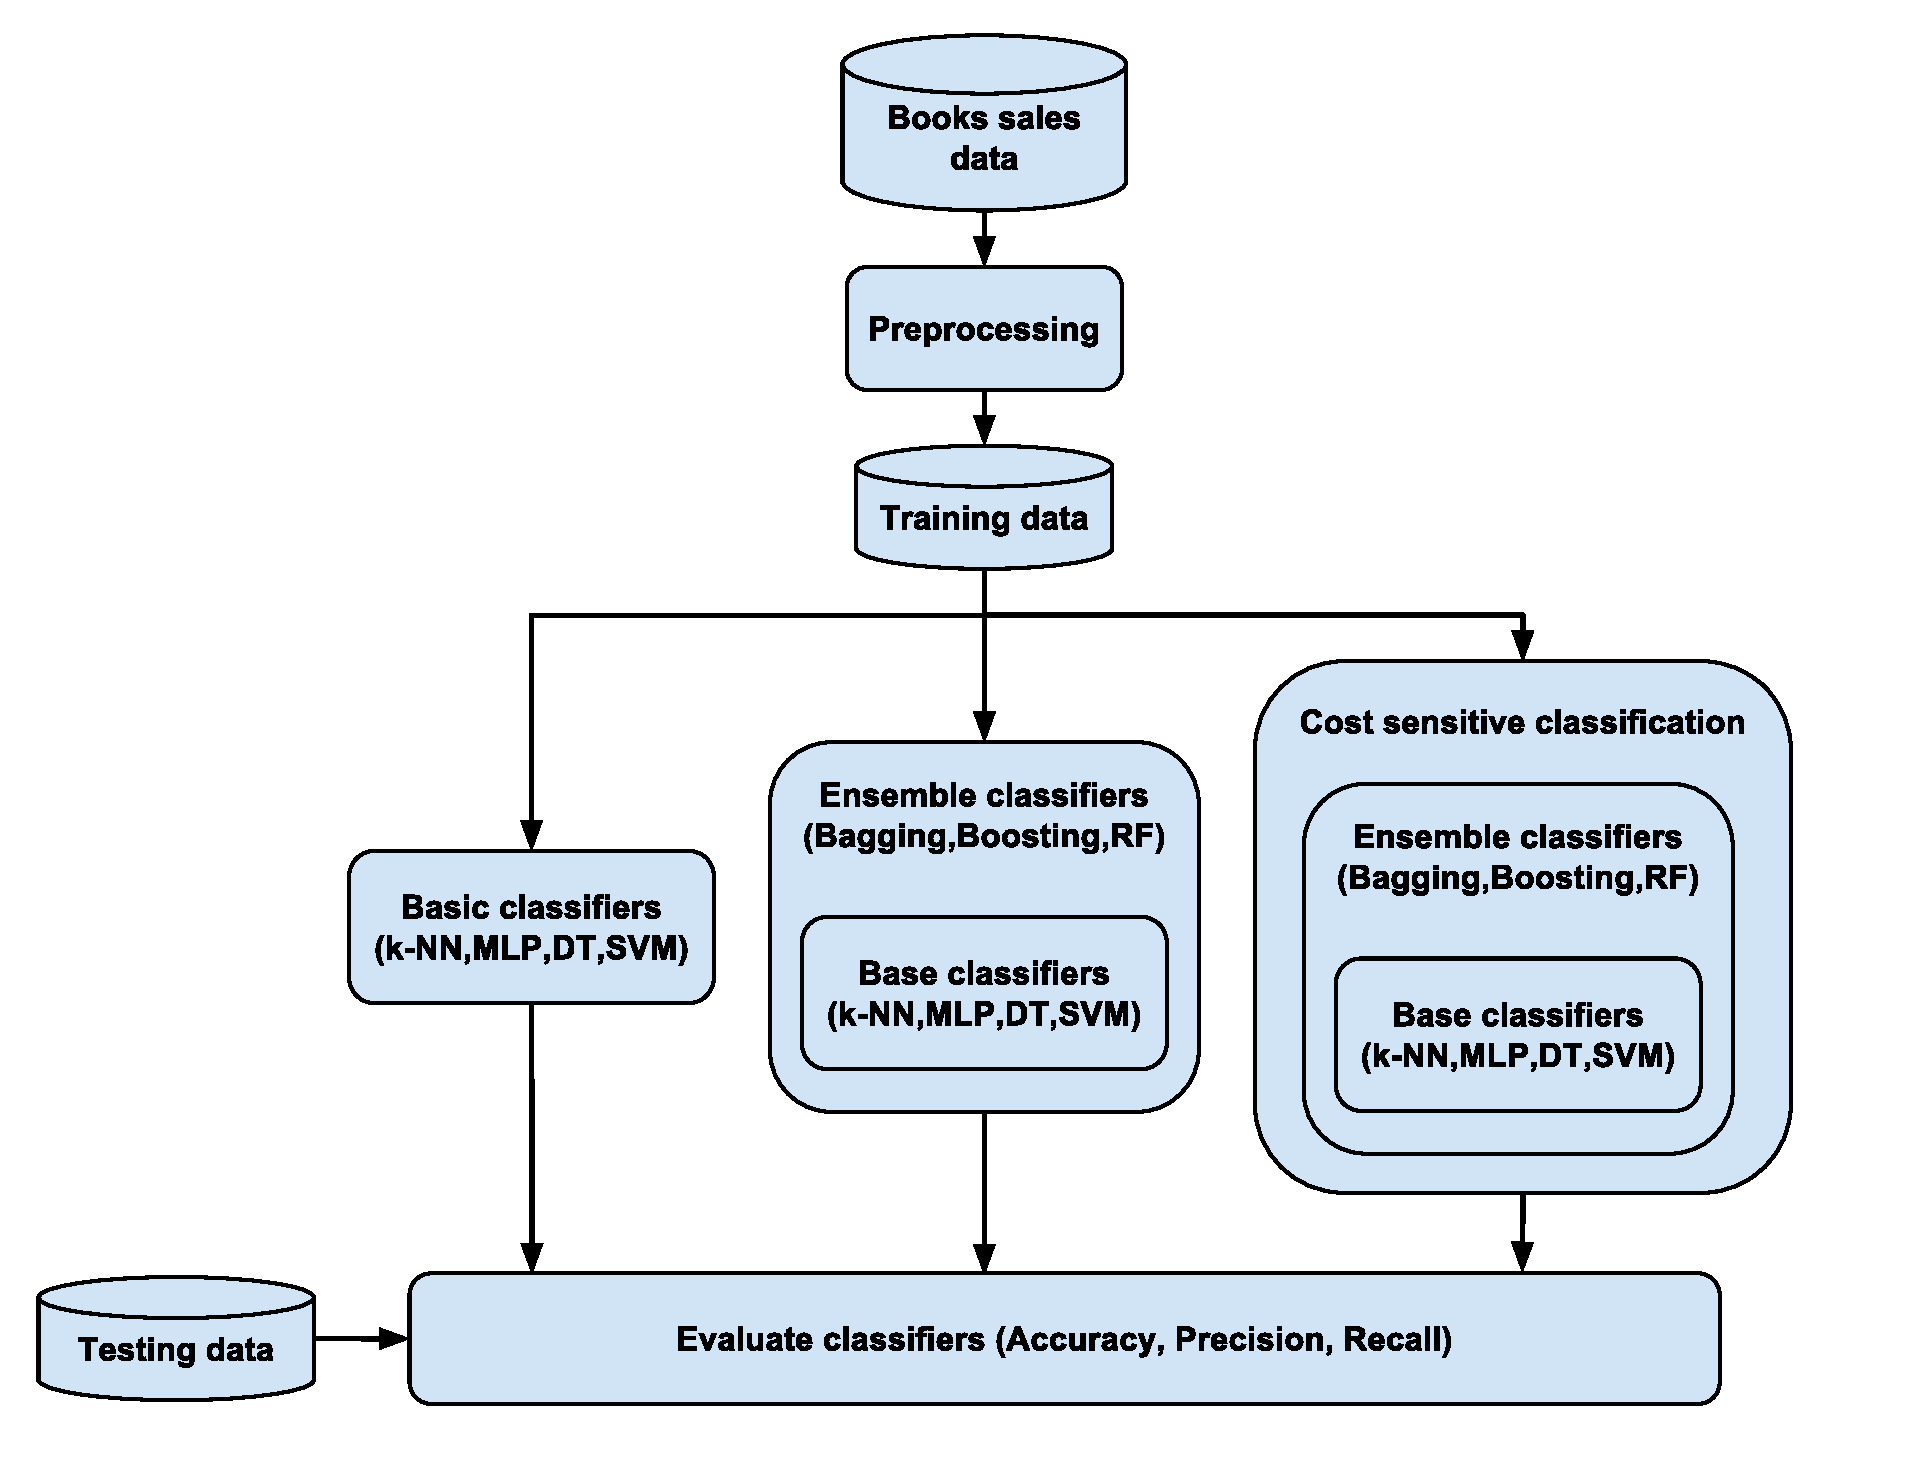
\includegraphics[scale=0.40]{books_methodology}
\end{center}
\caption{Proposed methodology.}
\label{fig:methodology}
\end{figure*}
% Antonio - I like this figure, however, it seems on it that the results of the basic classifier are used as 'starting point' of the ensembles, and the results of these methods are used in the cost sensitive classification... is this correct? Otherwise, maybe we should change the design of the figure. ;D
% Hossam: I have changed the figure as Antonio suggested ;)

%*******************************************************************************
%										MATERIALS AND METHOD
%*******************************************************************************
\section{Materials and methods}
\label{sec:materials}

%-------------------------- BASIC CLASSIFIERS --------------------------
\subsection{Basic classifiers}
\label{subsec:classifiers}

In order to show the need for more intelligent and complex classification models, basic and more common models are experimented and applied first. 
\begin{itemize}

\item \textbf{$k$-Nearest Neighbors ($k$-NN)}
The kNN \cite{Aha1991,Mitchell1997} method is an instance-based classifier in 
which unknown patterns/instances are classified by relating them to the labelled ones, using a distance measure or function, usually Euclidean or Minkowsky distances.

The algorithm is based on the idea that two patterns with a high distance between them are less likely to belong to the same class than two close ones.

In the simplest approach, for every unknown instance to classify, the algorithm finds its nearest neighbour (in the patterns space), and assigns the class of that neighbour to the unknown pattern.
However, it is more common to apply a more robust approach, in which $k$ neighbours are located, and thus, assigning the majority class of these instances to the unclassified pattern.

\item \textbf{Naive Bayes classifier (NB)}

This is a type of probabilistic classifier, based on the Bayes' Theorem \cite{AI-book_Bayes}, which considers a \textit{naive} (or strong) independence between the variables of the samples to be classified.

It is normally used as a baseline for comparison, because it usually yields competitive results in low computational time. Moreover, naive Bayes classifier shows a very good performance when there is considered a supervised training stage.

This method has a very good scalability, requiring a linear number of parameters to work, depending on the number of variables of the problem. These parameters are the mean and standard deviations of the variables of every class.
Thus, it just evaluates closed-form expressions, not needing to iterate to refine the solutions as most of methods do.


\item \textbf{J48 - Decision Trees (DT)}

This method is an implementation of the C4.5 classifier, which generates the so-called \textit{decision trees}. It was introduced in 1993 by Quinlan \cite{Quinlan1993} as an extension of the ID3 algorithm \cite{Mitchell1997}. 

The algorithm builds a decision tree using the attributes of the input patterns as nodes and considering its values for defining a decision in that node. Thus, for each node, the best attribute for splitting the training set is selected. The criteria for choosing one attribute is based on the difference of entropy (normalized information gain) obtained by every possible division. The one which yields the highest information gain is chosen as the best. This process is repeated for the subsequent data subsets, building subtrees. Normally, the decision tree is iteratively refined (or pruned) to maximize these gains and to avoid useless subtrees.


\item \textbf{Multilayer Perceptron Neural Network (MLP)}

It is an artificial neural network generally used for classification or 
approximation/regression problems \cite{Rosenblatt1962,Widrow1990}. It maps the input data onto an appropriate output, as a generalisation of the standard linear perceptron that uses several layers of nodes, called neurons. Each neuron consists of a linear combination of weighted inputs which is passed through a non-linear activation function to produce its output.

Thus, a MLP is able to solve linearly inseparable problems \cite{SteinwenderBitzer2003}. It is normally trained using a supervised learning 
technique called \textit{back-propagation}. This method was proposed by Werbos, Parker and Rumelhart et al. \cite{Werbos1974,Parker1985,Rumelhart1985}, and consists in updating the weights of the output layer neurons according to the obtained erroneous output. Then, the weights are updated inversely up to the input layer.
There are normally two hidden layers, as some works \cite{Lippmann1987,Bishop1996} demonstrated to be enough to 
create classifying regions of any kind.


\item \textbf{Support Vector Machines (SVM)}
SVM \cite{Cortes1995,Shevade2000} is a method which applies statistical learning theory. In classification problems, the algorithm searches for an optimal hyperplane that separates two classes, maximising the margin between them. 
This hyperplane is defined by a subset of training set samples, called support vectors.

This method is highly robust and reliable even if the space is highly dimensional and the problem is not linearly separable.

SVM has been successfully applied in forecasting and classification problems \cite{Cao2003,MinSVM05,Jari2008}.


\end{itemize}



%-------------------------- ENSEMBLE CLASSIFIERS --------------------------
\subsection{Ensemble classifiers}
\label{subsec:ensembles}

\begin{itemize}
\item \textbf{Bagging} 
Bagging which is called also Bootstrap aggregating is an ensemble meta-algorithm introduced by \citet{B1996}. Bagging works by training base classifiers (usually decision tree classifiers) based on generated new datasets from the original training dataset. The new generated datasets are drawn randomly with replacement in a size almost equal to the original dataset. The final classifier's output is based on aggregating the classifiers by taking a majority or weighted vote.


\item \textbf{Boosting} 
Boosting is an ensemble classification algorithm which was first proposed by \citet{schapire1990strength} in \citet{schapire1990strength}. Boosting is based on the idea that a set of weak classifiers can create a stronger one. In this work we adopt a powerful a variation of boosting called Adaptive Boosting or ''Adaboost'' for short \cite{FS1997}. Adaboost operates on a training dataset ${(x_{1},y_{1}),...,(x_{m},y_{m})}$ where each $x_{i}$ is a set of inputs belongs to some domain $X$ and each $y_{i}$ belongs to some label $Y$ assuming $Y$ is a binary class set $\{+1,-1\}$. 


During the learning process, Adaboost modifies the dataset by weighting its samples. These weights are updated every time a new classifier is trained to increase the focus on the difficult data instances. Consequently, the final generated classifier is a weighted combination of all trained base classifiers. According to many previous works, Adaboost is resistant to overfitting and it can outperform many other state-of-the-art classification techniques.


\item \textbf{Random Forest}
This method is based on the construction of a set of decision trees using a stochastic process over the basis of C4.5 algorithm. It was proposed by Breiman in \cite{Breiman2001} and aims to create independent and uncorrelated trees based on different and random input vectors, following the same distribution. 
The result is the average of the generated trees during the process.
\end{itemize}


%*******************************************************************************
%										COST SENSITIVE CLASSIFICATION
%*******************************************************************************
\section{Cost sensitive classification}
\label{sec:cost_sensitive_classification}

%------------------------ COST SENSITIVE LEARNING ------------------------
\subsection{Cost sensitive learning}
\label{subsec:cost_learning}

%------------------------ COST SENSITIVE CLASSIFICATION ------------------------
\subsection{Cost sensitive classification}
\label{subsec:cost_classification}


%*******************************************************************************
%										DATASET
%*******************************************************************************
\section{Dataset description}
\label{sec:dataset}


The obtained dataset contains collected information about 6083 different books produced by 209 publishers. Each book or pattern in the dataset is represented by 10 features as shown in Table \ref{tabla:params_pre_sales}. 


\begin{table*}
\caption{Pre-sales features and Sales level(Output class). } 
\label{tabla:params_pre_sales}
\begin{center}
\begin{tabular}{|c|l|l|c|c|}
\hline 
No. & Feature Name & Variable & Type & In/Out\\
\hline 
1 & retail price (when launched) & \texttt{ret\_price} & numerical & input\\
2 & main subject (code) & \texttt{subject1} & numerical & input\\
3 & bookbinding (code) & \texttt{binding} & categorical & input\\
4 & gifts (promotional books) & \texttt{gifts} & numerical & input\\
5 & units distributed as novelty & \texttt{distrib\_novelty} & numerical & input\\
6 & total number of points of sale & \texttt{tot\_points\_sale} & numerical & input\\
7 & total number of points of sale (1st year) & \texttt{tot\_points\_sale\_1st\_year} & numerical & input\\
8 & weeks on sale & \texttt{weeks\_sale} & numerical & input\\
9 & print run & \texttt{print\_run} & numerical & input\\
\hline 
\hline
10 & Sales level & \texttt{sales\_level} & categorical & output\\
\hline 
\end{tabular}
\end{center}
\end{table*}


The output variable which is the total sales is a categorical variable the represent the level of the quantity sold of a given book. Four categories are used to represent the total sales level: Low (L), Medium (M), High (H) and Very High (VH). Table \ref{table:freq} shows the ranges of total sales that correspond to each category along with the number of sold books that fall in. Discretization of the volume of sales was conducted with the aid of experts in the domain of editorial management business by defining the the four categories.

% Antonio - We must explain how did we obtain or 'define' these categories... an expert's opinion or so. ;D
% Hossam - I have added this to the latter paragraph. Please check.
 

Table \ref{table:freq} reveal more information about the nature of the dataset. We can notice that most of the investigated books are categorized as Low and Medium levels forming 26.8\% and 36.4\% of the dataset, respectively. High volumes of sold books that range from 300 up to 1000 are categorized as High volume of sales and form 24\% of the dataset. On the other hand, books that achieved more than 1000 sold copies are categorized as Very High and they form around 12.8\% of the dataset. Our focus in this study is to identify the more profitable categories which are High and Very High. However, since the latter category is much smaller than the other ones, we can describe our dataset as imbalanced dataset which makes the problem of identifying this category harder and more challenging.





\begin{table*}[ht]
\caption{Categories corresponding to total sales }
\centering{}%
\begin{tabular}{|c|c|c|c|}
\hline 
Category & Range of total sales & Count & Ratio\tabularnewline
\hline 
\hline 
Low & 0-60 & 1631 & 26.8\%\tabularnewline
\hline 
Medium & 61-300 & 2212 & 36.4\%\tabularnewline
\hline 
High & 300-1000 & 1460 & 24\%\tabularnewline
\hline 
Very High & $>$1000 & 780 & 12.8\%\tabularnewline
\hline 
\end{tabular}
\label{table:freq}
\end{table*}


%*******************************************************************************
%										EVALUATION MEASUREMENTS
%*******************************************************************************
\section{Evaluation measurements}
\label{sec:eval_measures}

To evaluate the developed classification models, first, we refer the confusion matrix shown in Table \ref{fig:confusionmatrix} which is considered as a basic source for evaluating any binary classification model. In our case which is a multiclass prediction problem, this matrix can be expanded with a row and column for each class to evaluate the multiclass classification models. Three measurements are used to evaluate the applied classifiers: accuracy rate, precision and recall. The accuracy rate simply measures the total number of correctly classified instances over the total number of instances $N$ as shown in Equation \ref{equation:acc}.

Precision is the ratio of the correctly classified instances as $i$ to the number of instances classified as $i$. On the other side, recall is the ratio of the correctly classified instances as $i$ to the number of actual $i$ instances. Precision and recall are given in Equation \ref{equation:precision} and \ref{equation:recall}, respectively.


\begin{figure*}[ht]
\begin{center}
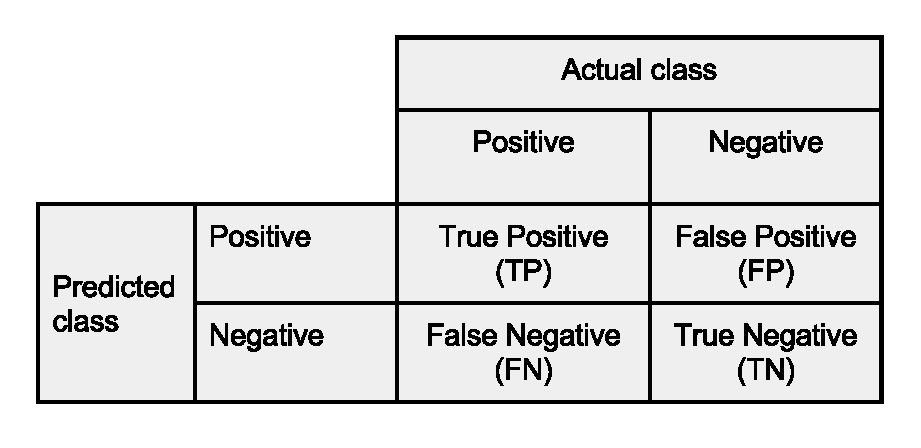
\includegraphics[scale=0.50]{Confusion-matrix}
\end{center}
\caption{Basic confusion matrix.}
\label{fig:confusionmatrix}
\end{figure*}

\begin{equation}
Accuracy=\frac{\sum_{i}C_{ii}}{N}
\label{equation:acc}
\end{equation}


\begin{equation}
Precision_{i}=\frac{C_{ii}}{\sum_{j}C_{ij}}
\label{equation:precision}
\end{equation}


\begin{equation}
Recall_{i}=\frac{C_{ii}}{\sum_{j}C_{ji}}
\label{equation:recall}
\end{equation}

\begin{figure*}[ht]
\begin{center}
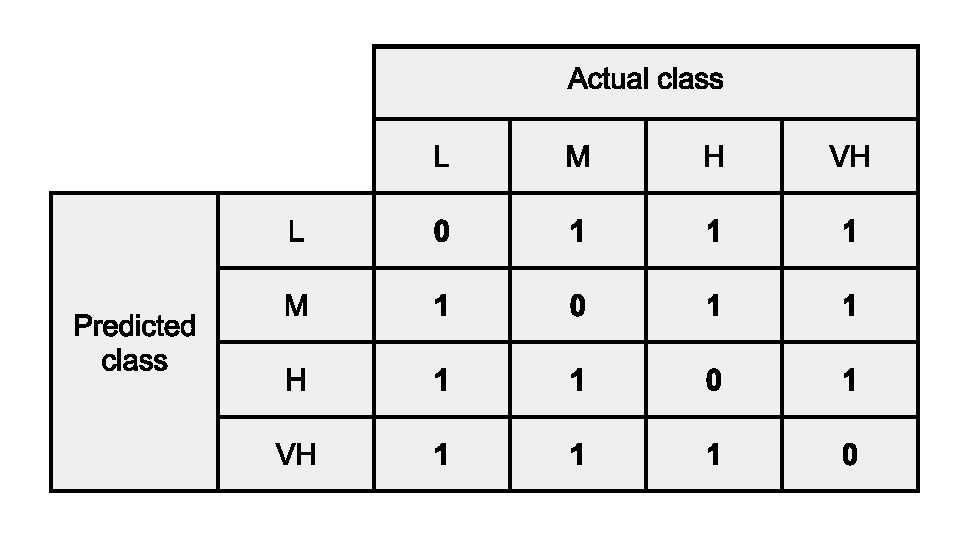
\includegraphics[scale=0.40]{Confusion-matrix-multiclass-default}
\end{center}
\caption{Default cost matrix.}
\label{fig:Default_cost_matrix}
\end{figure*}




%*******************************************************************************
%										EXPERIMENTS AND RESULTS
%*******************************************************************************
\section{Experiments and results}
\label{sec:experiments_results}

%This is just the first step of the experiments
% This table shows the average results of 10X10-folds experiments of the basic classifiers.
% It is impossible to calculate directly the average Precision and Recall for each class for multiclass problems in Weka Experimenter. So I have written a bash script to generate the row predictions utilizing Weka 3.9 developers version. Then I wrote another Python script to process these predicitons and calculate the precision and recall measurements as listed in this table.

In all experiments, 10-folds cross validation methodology is applied for training and testing the developed classifiers. Moreover, in order to generate statistically reliable results, the 10-fold cross validation is repeated 10 times with different partitioning seeds then the average and standard deviation are calculated for each evaluation metric.

In the first stage of the experiments the basic classifiers k-NN, NB, MLP, J48 and SVM are applied for predicting the sales level. The performance of some classifiers is highly affected by the initial values of their parameters. For this reason, initial experiment were conducted to tune the parameters of k-NN, SVM and MLP. For k-NN the best classification results were obtained with k=1. For SVM, a rough grid search was used, the value for the cost $C$ is set to 50 and $\gamma$  to 0.01. For MLP, the number of hidden neurons is set to (number of features+ number of output classes)/2.


The developed classifiers are assessed by measuring their accuracy and the precision and recall of each class label. Evaluation measures for all classifiers are shown in Table \ref{table:basic_classifiers}. It can be noticed that all classifiers have obtained very close accuracy ratios with a slight advantage for the MLP network with 71\% accuracy. In general, accuracy rates don't give an insight on how the classifier performs regarding each class. Therefore, precision and recall rates are examined for each class. Precision and recall values in Table \ref{table:basic_classifiers} show that J48 classifier achieved the highest recall value of 72\% for (VH) class with 74\% precision. The second best classifier for this important class is MLP with 68\% recall and 77\% precision. Having a look at the second important class which is (H), we can see that MLP has the highest recall with 65\% and a precision of 62\%. J48 comes second for the (H) class with a slight decrease in the recall value.



\begin{table}
\caption{Classification results using basic classifiers (without print-run)}
\centering{}%
\begin{tabular}{|c|c|c|c|c|c|}
\hline 
 & kNN  & NB  & J48  & MLP  & SVM\tabularnewline
\hline 
\hline 
$Accuracy$  & 0.69$\pm$0.0026 & 0.67$\pm$0.0008 & 0.7$\pm$0.004 & 0.71$\pm$0.0027 & 0.67$\pm$0.0012\tabularnewline
\hline 
\hline 
$Recall_{L}$  & 0.75$\pm$0.0044 & 0.86$\pm$0.0013 & 0.79$\pm$0.0071 & 0.78$\pm$0.0222 & 0.59$\pm$0.0035\tabularnewline
\hline 
$Precision_{L}$  & 0.78$\pm$0.003 & 0.73$\pm$0.0017 & 0.8$\pm$0.0049 & 0.8$\pm$0.0173 & 0.84$\pm$0.0025\tabularnewline
\hline 
\hline 
$Recall_{M}$  & 0.74$\pm$0.0034 & 0.66$\pm$0.0024 & 0.7$\pm$0.0072 & 0.71$\pm$0.0129 & 0.82$\pm$0.002\tabularnewline
\hline 
$Precision_{M}$  & 0.65$\pm$0.003 & 0.64$\pm$0.0007 & 0.68$\pm$0.0079 & 0.69$\pm$0.007 & 0.59$\pm$0.0012\tabularnewline
\hline 
\hline 
$Recall_{H}$  & 0.59$\pm$0.0047 & 0.53$\pm$0.0022 & 0.6$\pm$0.0099 & 0.65$\pm$0.0346 & 0.55$\pm$0.0016\tabularnewline
\hline 
$Precision_{H}$  & 0.62$\pm$0.0037 & 0.58$\pm$0.0017 & 0.62$\pm$0.0058 & 0.62$\pm$0.0109 & 0.63$\pm$0.0012\tabularnewline
\hline 
\hline 
$Recall_{VH}$  & 0.6$\pm$0.0073 & 0.53$\pm$0.003 & 0.72$\pm$0.0086 & 0.68$\pm$0.0336 & 0.61$\pm$0.0012\tabularnewline
\hline 
$Precision_{VH}$  & 0.79$\pm$0.0071 & 0.81$\pm$0.0032 & 0.74$\pm$0.0072 & 0.77$\pm$0.0212 & 0.78$\pm$0.0028\tabularnewline
\hline 
\end{tabular}
\label{table:basic_classifiers}
\end{table}


In the next stage of the experiments, the ensemble classifiers (i.e. RF, Bagging and AdaBoost) are applied and evaluated. For Bagging and AdaBoost, the base classifier is selected to be the J48 decision tree algorithm. This selection is for three reasons: first, the J48 algorithm achieved very competitive evaluation results in the previous phase. Second, J48 is much faster as a learning algorithm compared to the MLP network which was the second candidate. Third, tree induction algorithms are good candidates as base classifiers in bagging and boosting because support diversity among the learners. It is well known that tree induction algorithms are relatively unstable (i.e. weak) base learners, meaning that small changes in the training data lead to big changes in the developed models. 




\begin{figure*}

\centerline{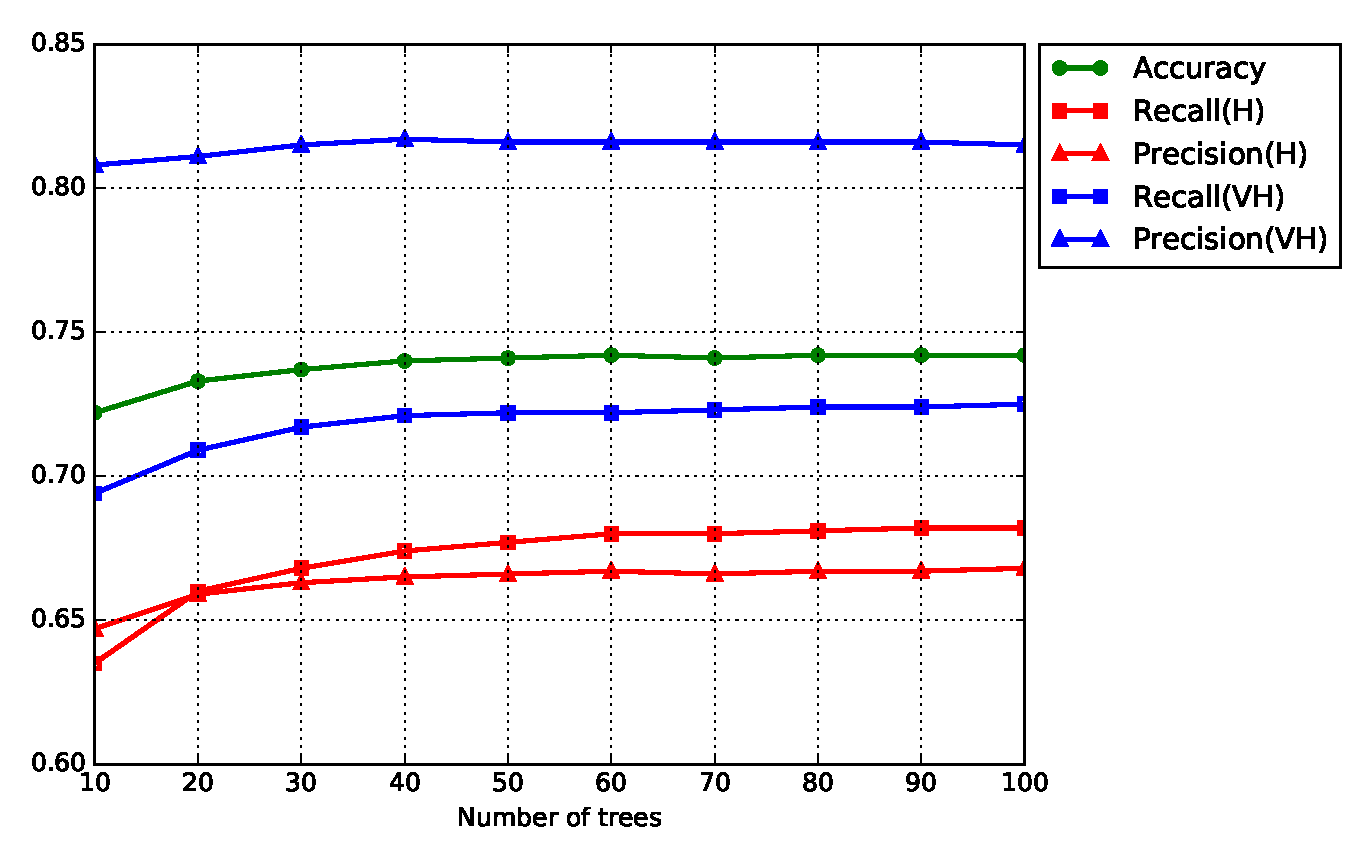
\includegraphics[scale=0.46]{RF}}

\caption{Performance of RF classifier over different number of trees.}
\label{fig:PerformanceRF}
\end{figure*}

\begin{figure*}
\centerline{
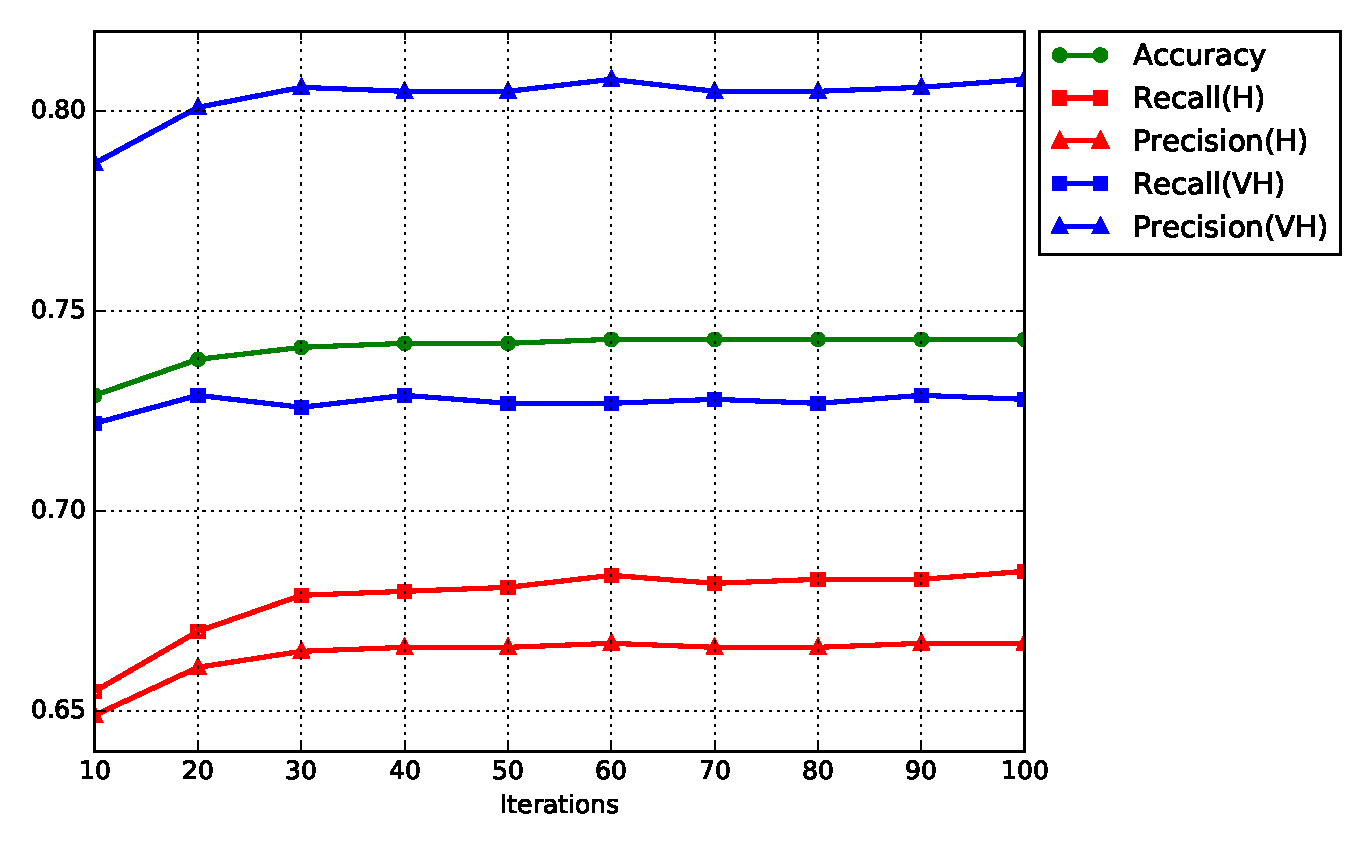
\includegraphics[scale=0.46]{Bagging}}

\caption{Performance of Bagging classifier over different number of iterations.}
\label{fig:PerformanceBagging}
\end{figure*}

\begin{figure*}
\centerline{
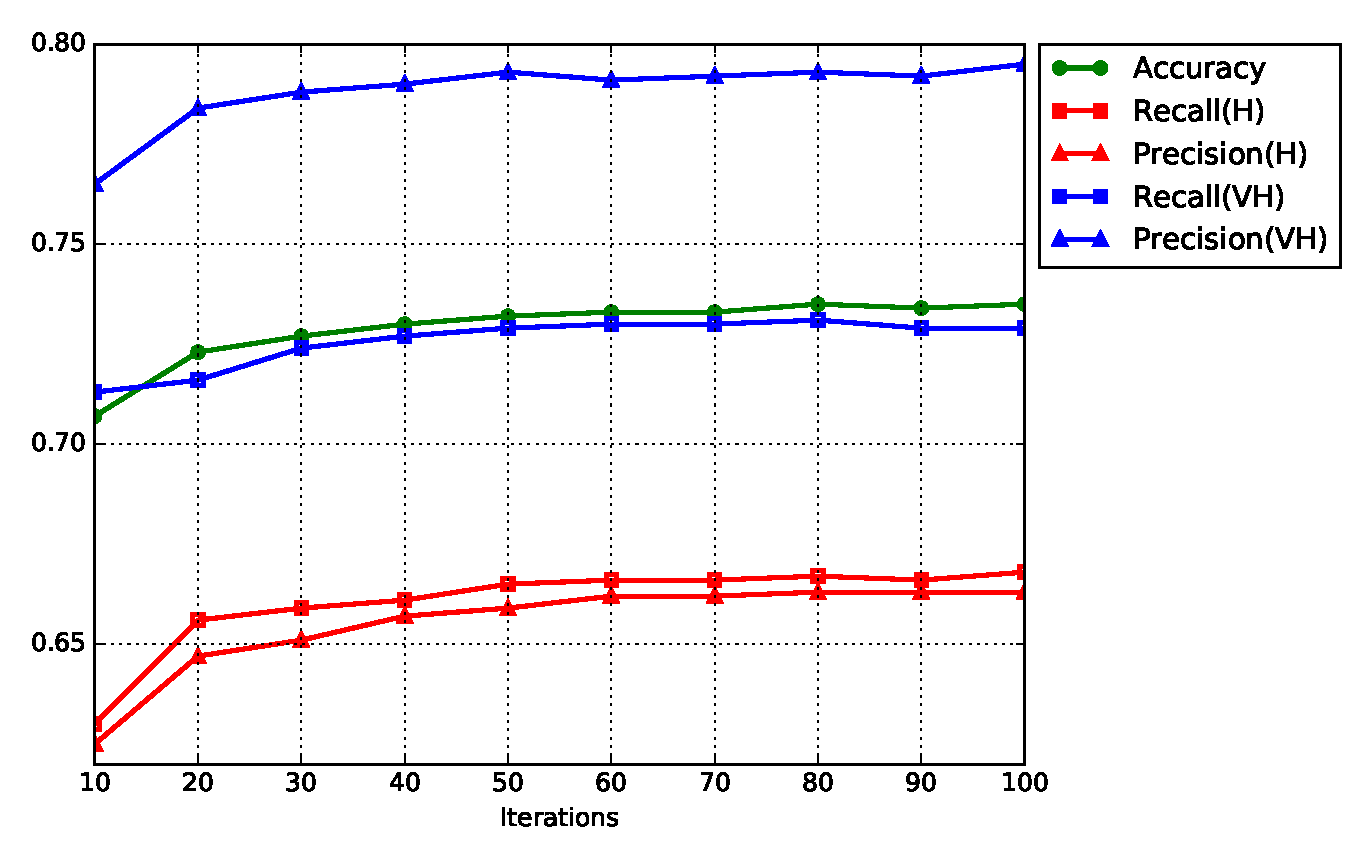
\includegraphics[scale=0.46]{Adaboost}
}
\caption{Performance of Adaboost classifier over different number of iterations.}
\label{fig:PerformanceAdaboost}
\end{figure*}

% Antonio - Just a comment about colors of the graphs. If one prints them in grey scale it cannot be distinguished for instance H and VH lines. ;)
% Hossam- I have updated all figure as you Antonio suggested and I have added also Low and Medium results to the figures.


\begin{table}
\caption{Classification results using ensemble classifiers (RF, AdaBoost and Bagging)}
\centering{}%
\begin{tabular}{|c|c|c|c|}
\hline 
 & RF  &  AdaBoost &  Bagging \tabularnewline
\hline 
 \hline $Accuracy$ & 0.741 $\pm$ 0.002 & 0.743 $\pm$ 0.0023 & 0.735 $\pm$ 0.0022 \tabularnewline 
 \hline 
 \hline $Recall_{L}$ & 0.796 $\pm$ 0.0038 & 0.793 $\pm$ 0.0038 & 0.792 $\pm$ 0.0048 \tabularnewline 
 \hline $Precision_{L}$ & 0.823 $\pm$ 0.0035 & 0.827 $\pm$ 0.0032 & 0.814 $\pm$ 0.0043 \tabularnewline 
 \hline 
 \hline $Recall_{M}$ & 0.748 $\pm$ 0.0033 & 0.75 $\pm$ 0.0029 & 0.738 $\pm$ 0.0038 \tabularnewline 
 \hline $Precision_{M}$ & 0.712 $\pm$ 0.0026 & 0.716 $\pm$ 0.0032 & 0.707 $\pm$ 0.004 \tabularnewline 
 \hline 
 \hline $Recall_{H}$ & 0.68 $\pm$ 0.0073 & 0.684 $\pm$ 0.0051 & 0.667 $\pm$ 0.0065 \tabularnewline 
 \hline $Precision_{H}$ & 0.666 $\pm$ 0.0037 & 0.667 $\pm$ 0.0029 & 0.663 $\pm$ 0.004 \tabularnewline 
 \hline 
 \hline $Recall_{VH}$ & 0.723 $\pm$ 0.0054 & 0.727 $\pm$ 0.0041 & 0.731 $\pm$ 0.0057 \tabularnewline 
 \hline $Precision_{VH}$ & 0.816 $\pm$ 0.0051 & 0.808 $\pm$ 0.0056 & 0.793 $\pm$ 0.0069 \tabularnewline 
\hline 
\end{tabular}
\label{table:ensemble_classifiers}
\end{table}

%*******************************************************************************
%										CONCLUSIONS AND FUTURE WORK
%*******************************************************************************
\section{Conclusions and Future Work}
\label{sec:conclusions_future_work}





%********************************************************************************
\section*{Acknowledgements}

This work has been supported in part by projects PreTEL (PRM Consultores - Trevenque S.L.), TIN2014-56494-C4-3-P and TEC2015-68752 (Spanish Ministry of Economy and Competitiveness and FEDER), and PROY-PP2015-06 (Plan Propio 2015, funded by the University of Granada, Spain).



%********************************************************************************
\bibliographystyle{elsarticle-num}
\bibliography{refs}

%----------------------------------------------------------------------

\end{document}
